\documentclass{standalone}

\usepackage{tikz}
\usepackage{standalone}
\usetikzlibrary{calc}

\begin{document}
    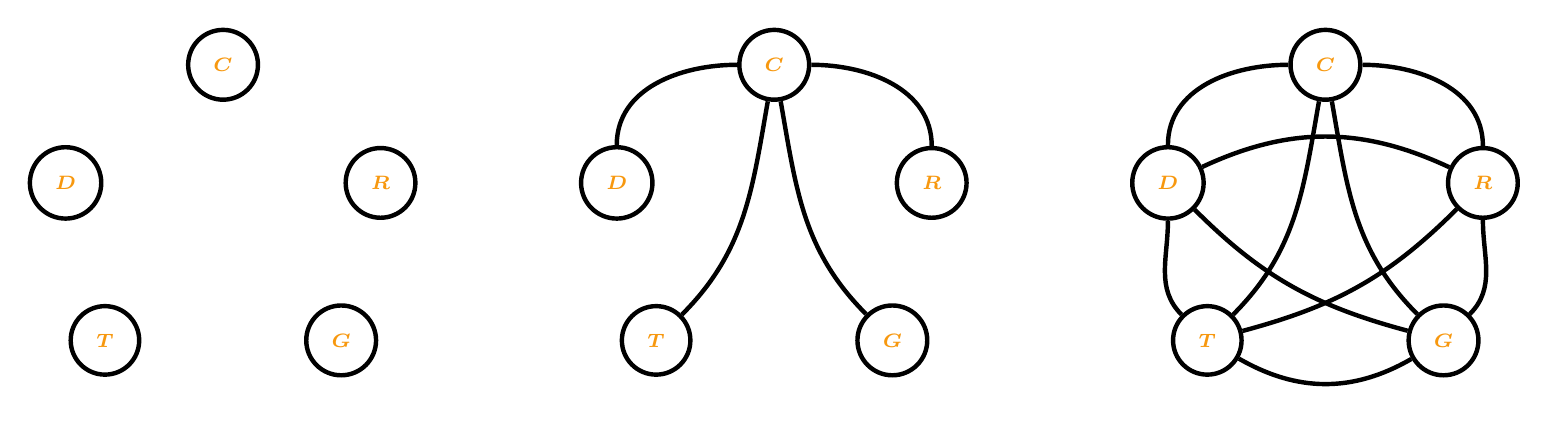
\begin{tikzpicture}

    \tikzstyle{state}=[minimum width=-0.2cm, font=\boldmath, inner sep=6pt];

    % , label=above:{\small{\textit{choose strategies}}}]
    \node[circle, draw, ultra thick] (0) at (0, 1.5) [state]   {  \scriptsize \textcolor{YellowOrange}{$C$}};
    \node[circle, draw, ultra thick] (1) at (-2, 0) [state]  {  \scriptsize \textcolor{YellowOrange}{$D$}};
    \node[circle, draw, ultra thick] (2) at (-1.5, -2) [state] {  \scriptsize \textcolor{YellowOrange}{$T$}};
    \node[circle, draw, ultra thick] (3) at (1.5, -2) [state]  {  \scriptsize \textcolor{YellowOrange}{$G$}};
    \node[circle, draw, ultra thick] (4) at (2, 0) [state]   {  \scriptsize \textcolor{YellowOrange}{$R$}};

    % , label=above:{\small{\textit{a player interacts}}}]
    \node[circle, ultra thick, draw] (5) at (7, 1.5) [state]   {\scriptsize \textcolor{YellowOrange}{$C$}};
    \node[circle, ultra thick, draw] (6) at (5, 0) [state]  {  \scriptsize \textcolor{YellowOrange}{$D$}};
    \node[circle, ultra thick, draw] (7) at (5.5, -2) [state] {  \scriptsize \textcolor{YellowOrange}{$T$}};
    \node[circle, ultra thick, draw] (8) at (8.5, -2) [state]  {  \scriptsize \textcolor{YellowOrange}{$G$}};
    \node[circle, ultra thick, draw] (9) at (9, 0) [state]   {  \scriptsize \textcolor{YellowOrange}{$R$}};

    \draw (5) edge[out=180, in=90, -, ultra thick] node [above] {} (6);
    \draw (5) edge[out=0, in=90, -, ultra thick] node [above] {} (9);
    \draw (5) edge[out=-100, in=45, -, ultra thick] node [above] {} (7);
    \draw (5) edge[out=-80, in=135, -, ultra thick] node [above] {} (8);

    % , label=above:{\small{\textit{players play against all}}}]
    \node[circle, ultra thick, draw] (10) at (14, 1.5) [state]   {\scriptsize \textcolor{YellowOrange}{$C$}};
    \node[circle, ultra thick, draw] (11) at (12, 0) [state]  {  \scriptsize \textcolor{YellowOrange}{$D$}};
    \node[circle, ultra thick, draw] (12) at (12.5, -2) [state] {  \scriptsize \textcolor{YellowOrange}{$T$}};
    \node[circle, ultra thick, draw] (13) at (15.5, -2) [state]  {  \scriptsize \textcolor{YellowOrange}{$G$}};
    \node[circle, ultra thick, draw] (14) at (16, 0) [state]   {  \scriptsize \textcolor{YellowOrange}{$R$}};

    \draw (10) edge[out=180, in=90, -, ultra thick] node [above] {} (11);
    \draw (10) edge[out=0, in=90, -, ultra thick] node [above] {} (14);
    \draw (11) edge[out=-90, in=135, -, ultra thick] node [above] {} (12);
    \draw (12) edge[out=-30, in=-150, -, ultra thick] node [above] {} (13);
    \draw (14) edge[out=-90, in=45, -, ultra thick] node [above] {} (13);

    \draw (12) edge[out=15, in=-135, -, ultra thick] node [above] {} (14);
    \draw (13) edge[out=165, in=-45, -, ultra thick] node [above] {} (11);

    \draw (10) edge[out=-100, in=45, -, ultra thick] node [above] {} (12);
    \draw (10) edge[out=-80, in=135, -, ultra thick] node [above] {} (13);

    \draw (11) edge[out=25, in=155, -, ultra thick] node [above] {} (14);

\end{tikzpicture}

\end{document}